% Set the author and title of the compiled pdf
\hypersetup{
	pdftitle = {\Title},
	pdfauthor = {\Author}
}

\section{Introduction}

We want computers to be able to interact with us, just like we interact with
them. This involves having them understand written text and voiced speech, as
well as being able to synthesise speech and text themselves. This includes
things like translation text and searching for key words in text.

A computer or a suite of programs that can do all of this is the goal for
Natural Language Systems. The catch is, that language is hard and complicated,
and to make computers do the things we want them to, we need to know how3
language works, and express this as an executable program.

Language is the representation of ideas, and the linkage of different ideas
together in such a way as to create new ideas. In order to understand any one
sentence (a sentence usually corresponds to one idea, event or action), we have
to understand what each symbol in the language means in isolation, and
understand how they're connected, and what the connections to do change the
meaning of the ideas.

Many factors affect the meaning of a sentence, but the connection between words
is always hierarchical, and we can represent sentences as trees:

\begin{figure}[ht]
  \centering
  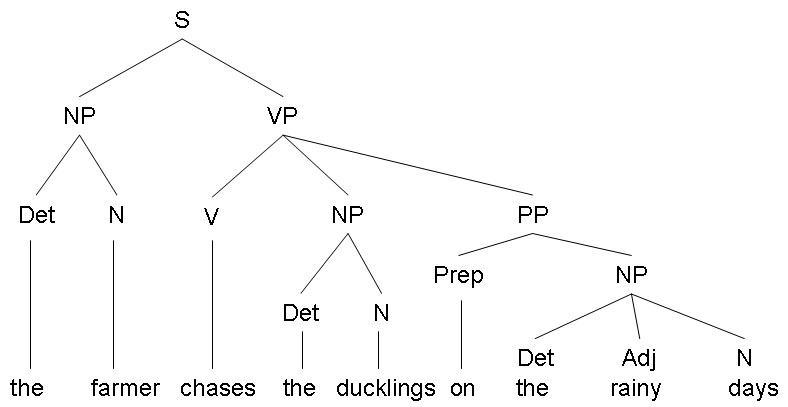
\includegraphics[width=0.55\textwidth]{images/phase-structure-tree}
  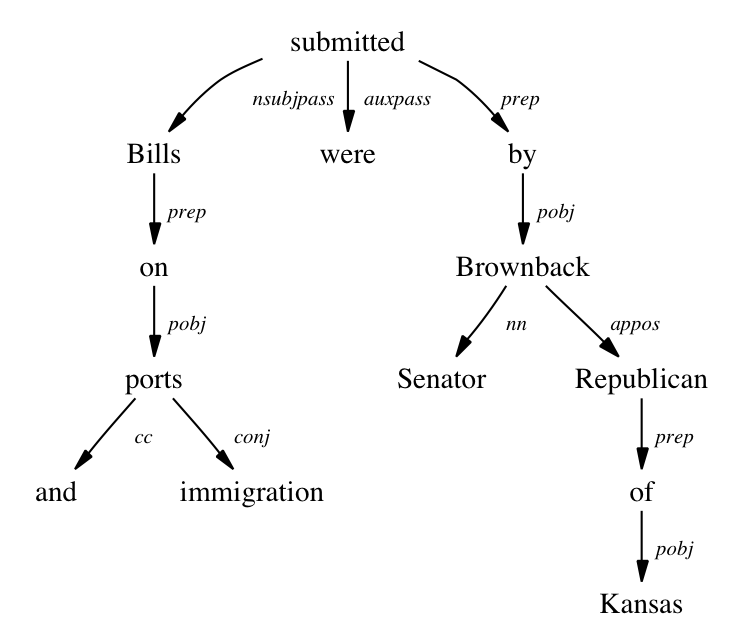
\includegraphics[width=0.35\textwidth]{images/dependency-tree}
  \caption{The left image is a phase structure tree, and the right image is a
  dependency tree.}
  \label{fig:trees}
\end{figure}

A parse tree is all well and good, but to a computer, this is only slightly more
useful than the original text. Though we have extracted some information out of
the text, we still just have a hierarchy of words, but we want a hierarchy of
ideas.

Having ideas instead of words allows us to infer more than what the text
literally says:

\begin{itemize}
  \item I'm fixing my motorbike $\rightarrow$ This person possesses a
  motorbike, and it is currently broken.
  \item The cake smells good $\rightarrow$ There is cake somewhere. Somebody is
  close enough to smell it.
\end{itemize}

But how can we do that?

\section{Structural analysis}

It is possibly to try and find out the meaning of a word simply by looking at
what letters it is made up of. One way to do this is to split a word into
\textbf{morphemes}, which are the most basic meaning-carrying components of a
word, and try to associate a meaning with each. For example \textit{undone}
could be split into \textit{un} and \textit{done}, and meaning associated with
each.

\subsection{Tries}

\marginpar{Tries are very handy datastructures for technical interviews, you
should read up on them an implement one!}

In order to examine the syntactic and semantic properties of the words, we need
to represent them in the computer. A common way to do this is with a
\textit{trie}:

\begin{wrapfigure}{r}{0.25\textwidth}
  \begin{center}
    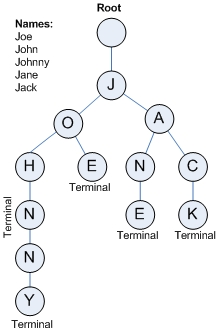
\includegraphics[width=0.24\textwidth,keepaspectratio]{images/trie}
  \end{center}
  \caption{A trie storing some names.}
\end{wrapfigure}

Tries are very memory efficient, since they if multiple words share the same
prefix, then the prefix is only stored once in memory. Tries have a lookup time
of $O(m)$, where $m$ is the length of the word, which is quite good, and is
better than a hash table in terms of speed in some cases. If you're stupid
enough to represent your dictionary as a list of words, then you can do a binary
search if its ordered (worst case $O(log(n) * m)$ comparisons (the $m$ comes
from having to possibly compare each character in the word)), or a linear search
if it isn't ordered ($O(m*n)$ in the worst case!).

\subsection{Spelling rules}

We want to understand why combining \textit{big} and \textit{est} produces
\textit{biggest} with an extra \textit{g}. Why isn't it \textit{bigest}? The
reason why we want to understand this, is so we can go from a word that we're
processing in text, and pick it apart into its components so we can better
understand it.

That is to say, we're going from \textit{biggest} to \textit{big} +
\textit{est}.

The format of the rules we're using in the course is as follows:

\marginpar{You can use \texttt{cX} and \texttt{vX} where \texttt{X} is an
integer, and \texttt{c/v} denotes a consonant or vowel inside the context
brackets.}

\begin{verbatim}
  [from] ==> [to]: [prevContext] _ [nextContext];
\end{verbatim}

For example, if we had a rule like:

\begin{verbatim}
  [g] ==> []: [g] _ [e,s,t];
\end{verbatim}

It would turn \textit{biggest} into \textit{big} + \textit{est}.

\subsection{Categorical descriptions}

Even if we find the meaning of every word by splitting it info morphemes, we
just end up with a collection of words that we know the construction of, but
we're still no closer to understanding a sentence.

In order to find the relationships between words in a sentence, we should use
the approach in Figure~\ref{fig:trees}, and try to fit the words into some tree
structure.

One way of doing this, is to specify lots of different forms that a sentence can
take. For example `noun verb noun' might describe a sentence such as `Todd
writes notes'. Providing that we have some \textit{prototype} for a sentence
that fits the words that we've been given, we can ascertain that we can in fact
make a sentence out of these words.

There is a better approach though. Each word in a sentence changes its meaning
in some way, and we can put words into buckets according to how the meaning of
the sentence is changed; for example, a verb specifies what kind of event is
happening. Having a verb on its own doesn't do us much good; we will know that
\textit{something} is happening, but not where, why, what, when etc. Verbs need
other parts of sentence around them to make them work.

We can treat each word as part of a jigsaw, specifying what other words or
phrases it needs in order to have meaning, and then fit the pieces together
according to some schema.

We need to specify a schema with which we can specify what different words require:

\begin{verbatim}
  <word> = <rules>
\end{verbatim}

The rules are their own language, which has a few rules. Brackets are
treated as they usually are in maths, and the only other special characters are
forward and backward slashes. These indicate whether a word or phrase should be
before or after the word.

\begin{verbatim}
  writes = (s\np)/np
\end{verbatim}

This indicates that the word `writes' needs a noun phrase (\texttt{np}) to its
right and then a noun phrase to its left to make a sentence (\texttt{s}).

With the right set of rules for each word, we can now parse sentences:

\begin{verbatim}
  writes = (s\np)/np
  Todd = np
  notes = np
\end{verbatim}

\begin{center}
  % Tabular centering hack
  \begin{tabular}{c}
    \begin{lstlisting}
      Todd        writes        notes
       np       (s\np)/np        np
                ---------------------
                        s\np
      -----------------------
                s
    \end{lstlisting}
  \end{tabular}
\end{center}

Here, the words `Todd' and `notes' are \textit{saturated} since they don't
require anything else to make them into complete `items'. `writes' is
unsaturated, since it needs other stuff to make it into a complete item. Word
rules of these kind are called \textbf{Categorical Descriptions}.

\subsection{Morphology}

Now we've figured out how to decompose a word into morphemes using spelling
rules, and we can fit these words into a sentence. However, we also want to know the precise meaning for each word (this helps when arranging them in a sentence too). We can do this by looking at each morpheme.

There are two types of morphology that we're going to look at:

\begin{description}
  \item \textbf{Inflectional morphology}\\
    This is when the stem of the word is incomplete, and other morphemes 
    provide more information to specify exactly what we mean:

    \begin{itemize}
      \item `sing' + `ing' = verb + present participle
      \item `work' + `ed' = verb + past participle
      \item `work' + `' = noun + singular
    \end{itemize}

  \item \textbf{Derivational morphology}\\
    This is where the meaning of the stem is significantly changed by other 
    morphemes. For example, `smelly' could be combined with `er' to give 
    `smellier', or `est' to give `smelliest'. Obviously we need spelling rules 
    to do this correctly!
\end{description}

We need a way to specify what words can have what suffixes/affixes. For example,
`conscript' can be combined with `tion' to give `conscription', but not `ly' to
give `conscriptly'.

Furthermore, there are spelling rules concerned with adding bits onto words; as
we saw before, `smelly' becomes `smellier', not `smellyer'. We will come across
this later though.

It turns out that composing morphemes is similar to composing words. We can use the same notation:

\begin{verbatim}
  'conscript' = noun>agr
  'conscript' = verb>tns
  'tion' = (noun>agr)<(verb>tns)
  'ing' = tns
  'ed' = tns
  's' = agr
  '' = agr
\end{verbatim}

These descriptions allow you to construct the following words:

\begin{mymulticols}
  \begin{itemize}
    \item conscript (noun)
    \item conscripts (noun)
    \item conscription (noun)
    \item conscriptions (noun)
    \item conscripting (verb)
    \item conscripted (verb)
  \end{itemize}
\end{mymulticols}

However, the rules are not perfect, and will also allow you to make:

\begin{mymulticols}
  \begin{itemize}
    \item conscriptingtion (noun)
    \item conscriptedtion (noun)
    \item conscriptingtions (noun)
    \item conscriptedtions (noun)
  \end{itemize}
\end{mymulticols}

We can also make rules cancel out. If we have a rule that is `verb$>$tns' and
another that is `tns$>$agr' then we can make a `verb$>$agr' from them.

To see a worked example of these rules, and how they're applied, look on slides
$64-110$ in the
\href{http://studentnet.cs.manchester.ac.uk/ugt/2015/COMP34411/COMP34411.pdf}
{course notes}.

One thing that is important to note, is that we can process words from left to
right, and don't have to back-track. This means that processing is in linear
time, which is fantastic (though we need a big dictionary of words, which is
rather less fantastic).

\subsection{Unknown words}

Now we can read in a sentence, parse each word and extract the relations between
the words to produce a meaningful parse tree, great! But\dots what if we
don't have a word in the input sentence in our dictionary? We won't be able to
fit it into our parse tree since it won't have any meaning to us. Looking at the
morphemes doesn't tell us too much; having `ing' at the end means that a word is
probably a verb and is in the present tense, but doesn't tell us what's actually
going on.

There are two different classes of classes of words \textit{open} and
\textit{closed}. Open classes are verbs, adjectives, nouns etc where there are
lots of them and you can easily add more (new nouns are created all the time).
Closed classes are things like prepositions (`in', `on'), and auxiliaries (`be',
`have', `would') where you rarely if ever get new words being added.

So, if we cannot recognise a word using the morphological rules we used before,
then we should \textbf{back off} to using a more robust but less accurate
strategy. Lets define exactly what robust and accurate mean:

\begin{description}
  \item \textbf{Robust}\\
    This is when a system always gives an answer, even if the answer might be 
    wrong. It's sometimes a good idea have a robust system, since then you can 
    always take \textit{some} action.
  \item \textbf{Accurate}\\
    An accurate system always gets the answer `right' when asked a question.
\end{description}

A common strategy in Natural Language Processing is to use a system that is
highly accurate but less robust, but fall back on a less accurate but more
robust system when the first doesn't give an answer.

So, we need to build a robust word recogniser for unknown words. To do this, we
need to know what word it is, and what part of speech tag it has (noun, verb
etc).

\subsubsection{Stemming}

If you were to come across the word `blodge', you probably wouldn't know what it
means (although there are, as always a number of definitions in the
\href{http://www.urbandictionary.com/define.php?term=blodge}{Urban Dictionary}).
If a word like `blodge' were to appear in the middle of a sentence, you could
probably still extract some information from it:

\begin{itemize}
  \item I went to blodge $\rightarrow$ Blodge is a place.
  \item I went to blodged it $\rightarrow$ Blodging is a thing you can do.
    The blodging happened in the past.
  \item The car was blodge $\rightarrow$ You can describe something as having 
    the property/quality `blodge'.
\end{itemize}

The \textbf{Porter Stemmer} is a set of rules that tell you what bits of a word
you can remove to get the stem of the word that is common to all forms of the
word. If we run the porter stemmer on `blodge', `blodging' and `blodged', then
we get the stem as `blodg'. Now we can at least identify all instances of
`blodg*' as the same word.

\subsection{Part of speech tagging}

When we look up a word in a dictionary, we get something like this:

\begin{figure}[H]
  \centering
  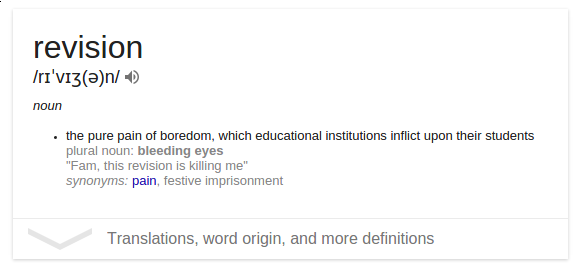
\includegraphics[width=0.75\textwidth]{images/revision-definition}
  \caption{A dictionary definition of the word `revision'.}
  \label{fig:revision-definition}
\end{figure}

Not only does a dictionary give us the definition of a word, but it also give us
its part of speech tag. In the case of Figure~\ref{fig:revision-definition} it
is a noun. We need the POS tag in order to work out how words are related to
each other, so we can put them in their proper place in a parse tree.

There are a number of ways to do part of speech tagging (this is what I'm doing
for my third year project, and it's a rabbit hole that you don't want to go down
if you're trying to revise for exams). Here are the ones you need to know for
this course:

\marginpar{One thing to be aware of with using corpuses, is that they are 
often ordered. If you use the first $N$ million words for training and the 
next $M$ million for testing, then you could end up with disastrous results, 
because different areas of the corpus will be about different genres, and 
will contain different words.}

\begin{description}
  \item \textbf{Dictionary look up}\\
  The easiest way to do POS tagging (but also the worst), is to get a big
  massive dictionary, and find the part of speech tag for each word. Then, when
  you need to tag a word, then you just look it up in your big list.

  However, you need lots and lots and lots of words to do this, and getting the
  tags for all of the words is a big task. Furthermore, if we're trying to
  handle unknown words, then by definition, we've not seen them before and they
  won't be in our dictionary.

  Obviously, the bigger your list of words, the fewer words you'll need to
  handle. The British National Corpus has 100 million words in, which is in the
  right ballpark, but it is poorly tagged (the error rate is above 1\% in
  parts). Other corpuses are available, but are either smaller, or you have to
  pay for them. In order to use the BNC (or any corpus) as a dictionary, you
  count how many times each word is tagged with each part of speech tag, and
  then assign the most common tag.

  There are two main advantages to this method; first of all, it's really
  simple, and computationally easy. Using a sensible hash table, lookup is
  $O(1)$ and training is $O(n)$. It's so fast that the bottleneck is usually the
  IO operations of reading (and decoding) the corpus. The second advantage, is
  that you get alternative tags for words. A word might be in the corpus 50
  times as a verb, but 20 times as a noun, and you can use this information in
  your processing.

  As a \textbf{backoff} technique, you can also keep track of the POS
  probabilities for the last $n$ letters of the word, so if the word isn't in
  your dictionary, you can use the last $n$ letters of it to determine what tag
  to assign.

  %TODO: Sefine precision and recall somewhere

  \item \textbf{Transition probabilities and HMM's}\\

  HMM's use probabilities and context to determine what tag a word should get.
  To train a HMM, we collect statistics on what part of speech tags
  \textit{follow and precede} other ones. For example, the probability of a noun
  being followed by another noun might be quite high, because of names (e.g.
  Todd Davies), and adjectives usually lead onto nouns, or other adjectives
  (e.g. hungry bored Todd).

  These are called \textbf{bigram} probabilities (because you have information
  about following and preceding tags). A HMM based POS tagger works as follows:

  \begin{itemize}
    \item For each word, use a corpus to calculate how likely it is to belong 
    to each class (just like we did for the dictionary look up approach). These 
    are the emission probabilities.
    \item For each tag that we have found that might correspond to a specific 
    word, look at the tag we assigned to the previous (and possibly next) word(
    s) and use the transition probabilities to choose the most likely tag.
  \end{itemize}

  We want to find the most likely sequence of tags for the whole sentence, which
  is why the hidden markov model works well. However, training can be slow and
  its hard to make use of the backward transition probabilities.

  \marginpar{I think this is more important for the POS tagging part of the
  course than HMM's are.}

  Alternately, you can use no HMM at all, by using a function to evaluate the
  best next tag:

  \[
    \begin{split}
    F(&dict(Word, tag_i),\\
      &\sum_k(P(tag(prevWord) = tag_k) \times P(tag_k \rightarrow tag_i)),\\
      &\sum_k(dict(nextWord, tag_k) \times P(tag_i \leftarrow tag_k)))
    \end{split}
  \]

  You can define $F$ to be anything, but in the course notes:

  \[
    F(dictProbability, forward, backward) = \sqrt{dictProbability} \times 
      (forward + backward)
  \]

  \item \textbf{Transformation Based Learning}\\
  \label{brill-rules}

  \marginpar{This is the subject of my third year project, when I've finished 
  it, I might remember to update these notes with a link to the code/my 
  dissertation.}

  Doing statistical tagging is pretty tedious, and requires a lot of text. Is
  there another way of doing POS tagging? Maybe one that could require less
  data?

  This is very possible, as was demonstrated in
  \href{http://dl.acm.org/citation.cfm?doid=974499.974526}{Eric Brill's PhD
  thesis} in 1995. The idea is to have a \textit{base tagger}, which is your 
  first guess at what the tag is (this is any POS tagger, like the ones above 
  for example), and then have rules that can correct mistakes in the output.

  This presents its own problems though. For example, how do you generate 
  rules? The solution is this:

  \begin{enumerate}
    \item Tag a small part of a corpus by hand, so the tags are 100\% (or very 
    close to it) accurate.
    \item Then you get come up with a set of rule \textit{templates}. Templates 
    (in this course) are of the form
    \texttt{\#name(entity1, entity2, entity3): oldTag > newTag if condition;} A 
    set of templates looks something like this:
    \begin{itemize}
      \item \texttt{\#t0(T1,T2): T1 > T2 if tag[0] = T1}\\
        Change tag T1 to tag T2 in every instance.
      \item \texttt{\#t1(T1,T2,T3): T1 > T2 if tag[-1] = T3}\\
        Change tag T1 to tag T2 if the previous tag was T3.
      \item \texttt{\#w0(T1,T2,W1): T1 > T2 if word[0] = W1}\\
        Change tag T1 to tag T2 if the current word is equal to W1.
    \end{itemize}
    \item Tag the corpus with the base tagger (something like a dictionary 
    lookup tagger, or transition probability tagger) plus any rules you've 
    generated so far, and then find the errors that it made. For every error,
    \textbf{instantiate a rule based on the context of the error}.
    \item Now you have lots of rules, you score each one by how many times it 
    would have made a good change, and how many times it would have made a bad 
    edit if you ran it on the whole corpus.
    \item Select the top rule, and run steps 3-4 again until you have enough 
    rules.
  \end{enumerate}

  I'm not sure if I like the format of the rule templates here, since they
  require you to specify that you're turning one specific tag into another. An
  example of an instantiated rule is:

  \texttt{\#t0(UN,NN,UN): UN > NN if tag[0]=UN;}

  This says turn every `UN' into a `NN'. What if we wanted to turn any tag into
  a `NN' if it was preceded by a `UN' though? We couldn't do this with this
  specific rule set, unless you had wildcards or something, e.g.:

  \texttt{\#t1(*,NN,UN): * > NN if tag[-1]=UN;}

  When you're assigning a score to each rule, you should give a gross score and
  a net score. The gross score is how many problems the rule would fix, but the
  net score is how many problems it would fix minus the number of correct
  taggings it wrongly breaks. You might end up with something like this:

  \begin{center}
    \begin{tabular} {|c|c|c|}
      \hline
      Rule ranking & Gross & Net\\ \hline
      1 & 500 & 300\\ \hline
      2 & 450 & 240\\ \hline
      3 & 412 & 234\\ \hline
      4 & 375 & 121\\ \hline
      5 & 297 & 100\\ \hline
      $\vdots$ & $\vdots$ & $\vdots$\\ 
    \end{tabular}
  \end{center}

  A brill tagger isn't really a part of speech tagger on its own, but it does go
  a long way to making existing POS taggers better. Depending on the
  characteristics of the base tagger, you can get anywhere from half a
  percentage extra accuracy, to a full ten percent extra. Remember though, if
  the base tagger is already 98\% accurate, half a percent is a big improvement!
\end{description}

\paragraph{Confusion matrices}

No matter how good our POS tagging algorithms are, they're always going to get
\textit{something} wrong. Confusion matrices are a way to spot common errors
that our taggers make. It is a table showing the correct tags along one side,
and the tags the POS tagger came up with along the other. Something like in
Table~\ref{table:conf-matrix}.

\begin{table}[h]
  \centering
  \begin{tabular}{|c|c|c|c|c|}
    \hline
        & NN  & VB  & PUN & $\dots$\\ \hline
    NN  & 80  & 4   & 0   & $\dots$\\ \hline
    VB  & 12  & 74  & 1   & $\dots$\\ \hline
    PUN & 0   & 0   & 12  & $\dots$\\ \hline
    $\vdots$ & $\vdots$ & $\vdots$ & $\vdots$ & $\ddots$\\ \hline
  \end{tabular}
  \caption{A sample confusion matrix. Along the top is the number of `correct' 
  tags, along the side is the number of tags we predicted.}
  \label{table:conf-matrix}
\end{table}

Apart from using them to gloat about your awesome POS tagger to your natural
language systems friends, confusion matrices are useful for improving the
accuracy of your tagger. If you have multiple taggers, each with a different
confusion matrix, then you can use the values in the matrix to determine which
one tagger to believe on any word.

If Tagger A says a word is a noun, but Tagger B another says its a determiner,
then what do you do? You can look at the confusion matrix, and see that $93\%$
of the time, the Tagger A gets nouns right, but $98\%$ of the time Tagger B gets
determiners right, then you should go with Tagger B. It's kind of like if you
herded a load of lecturers into a room and started asking them CS questions. If
you asked a question about complexity theory, you're more likely to get a good
answer from somebody who teaches an advanced algorithms course than you are from
somebody who teaches a UX course.

\marginpar{NLP stands for Natural Language Processing, not Neuro-Linguistic
Programming...}

\paragraph{Special cases} Sometimes, a POS tag is very ambiguous; the kind of
thing that would have linguists arguing for ages trying to determine which was
right. In these cases, we don't want to assign the wrong tag and mis-lead
whatever system is using our tags further down the NLP pipeline. As a solution,
we could define some special cases (the word `that' is hard to tag, for
example), and if we're not sure about a tag, make the tag equal to the word.
This technique is called \textbf{underspecification}.

\subsection{Regular expressions}

Now we can find the part of speech tag for any word (or at least give a good
guess for it), we can start to assign structure to the sentence. Given the words
of a sentence and their part of speech tags, using a grammar to parse sentences
can be done in $O(n^3)$ time \textbf{so long as lecixal ambiguity and out- of-
place words are ignored}. The trouble with this, is that both these things
really matter, and an algorithms that doesn't work, isn't very much use at all.

So, when our grammar does break down in those cases, we need to be able to
\textit{back off} to another more robust technique. This could be regular
expressions. Say a noun phrase is made of an optional determiner, zero or more
adjectives and then a noun:

\begin{verbatim}
  NP = DET? ADJ* NOUN
\end{verbatim}

A verb phrase is made of a verb and either one or two noun phrases, while a
sentence is made of a noun phrase and a verb phrase:

\begin{verbatim}
  VP = (VERB PREP? NP) | (VERB PREP? NP NP)
  s = NP VP
\end{verbatim}

Given a string that was tagged (correctly), you could apply the regular
expression to the string to get the sentences:

\begin{center}
  % Tabular centering hack #2
  \begin{tabular}{c}
    \begin{lstlisting}
      The reader wishes for    a   long break.
      --- ------ ------ ---    -   ---- -----
      DET NOUN   VERB   PREP  DET  ADJ  NOUN
      ----------              --------------  
        NP                        NP
                 --------------------
                         VP
       ---------------------
                 s
    \end{lstlisting}
  \end{tabular}
\end{center}

If we tag a sentence from the BNC, and run it through a simple regex, then we
can efficiently and effectively parse the sentence. First we need to go from the
BNC tags (they have different types of nouns, adjectives etc, looking like `NN4'
for a type 4 noun) to more sensible tags:

\begin{verbatim}
  'noun': 'NN.'
  'adj': 'AJ.'
  'det0': '(AT|D.).'
  ...
\end{verbatim}

Then we need to recognise phrases:

\begin{verbatim}
  'nmod': 'adj|noun'
  'np0': '((det0? nmod* noun)|name|pron)'
  ...
\end{verbatim}

Then you end up with something like:

\begin{center}
  % Tabular centering hack #2
  \begin{tabular}{c}
    \begin{lstlisting}
      <NP><DET>The</DET><NOUN>reader</NOUN></NP><VP><VERB>wishes</VERB>
      <PREP>for</PREP><NP><DET>a</DET><ADJ>long</ADJ><NOUN>break</NOUN>
      <NP></VP><PUN>.</PUN>
    \end{lstlisting}
  \end{tabular}
\end{center}

\marginpar{Regexes also don't give you alternate options for parsing. They give 
you one answer (i.e. `the string you gave matches this structure'), or no answers 
at all.}

This is good, and reasonable fast when your regex is small, but unfortunately,
the regex has to get quite large for the output to be a correct parsing of the
sentence, and then the regex parsing is quite slow. Furthermore, the output
looks horrible, and since regex matching is an opaque thing, you can't debug it
very well!

Ultimately, you can recognise a sentence and its structure using regexes, but
it's hard to make them parse a sentence just how you like it. Regexes aren't the
exactly easy to come up with, and in order to properly define a sentence
structure we need recursion (a noun phrase may contains another noun phrase).
Unfortunately, regexes don't know about recursion, so we need to cascade them:

\begin{verbatim}
  'a': 'c b'
  'b': 'a d'
  ...
\end{verbatim}

\subsection{Supertagging}

%TODO: WTF is supertagging

Make me a pull request to fill in this section, do it now!

\url{http://github.com/Todd-Davies/third-year-notes}{}

%TODO: Page 193 onwards

\subsection{Deterministic dependency parsing}

Using a regex to parse the structure of a sentence isn't widely done. In
practice, the way that gets the best results is to use a non-deterministic
algorithm. However, (as you may know all to well from \texttt{COMP36111}) non-
deterministic algorithms don't run very quickly at all on deterministic
computing machines, and will often exhibit an exponential runtime.

We therefore want to find a deterministic algorithm to extract a sentence
structure. When we're thinking about this, we want to optimise for three things:

\begin{itemize}
  \item Accuracy - get the correct answer
  \item Robustness - at least \textit{give} an answer
  \item Speed - try to have a polynomial time complexity
\end{itemize}

A good approach is to try and make a system that has a good accuracy, then
compromise until the other two criteria are satisfied too.

To parse a sentence into a structure, we can recognise the following points:

\begin{itemize}
  \item Each word has exactly one parent (except the root word)
  \item You can draw arrows between words in a sentence, and none of the arrows 
  will cross (see Figure~\ref{fig:dependency-relations} for an explanation).
\end{itemize}

\begin{figure}[h]
  \centering
    \begin{subfigure}[b]{0.55\textwidth}
    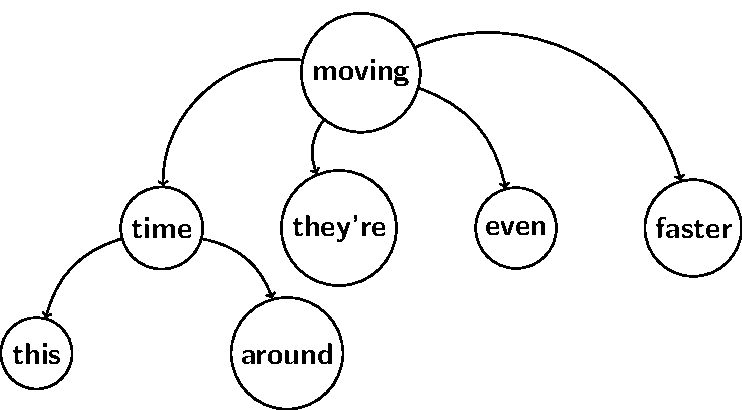
\includegraphics[width=\textwidth]{diagrams/dependency-tree}
    \caption{}
    \label{fig:dependency-tree}
  \end{subfigure}

  \begin{subfigure}[b]{0.55\textwidth}
    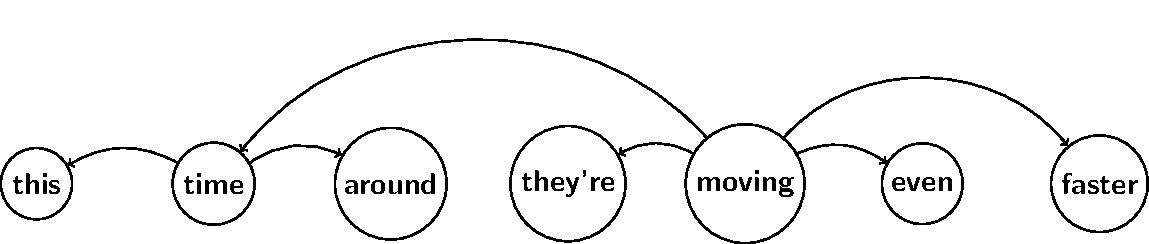
\includegraphics[width=\textwidth]{diagrams/dependency-relations}
    \caption{}
    \label{fig:dependency-relations}
  \end{subfigure}

  \caption[Two dependency representations]{(a)A dependency tree for the sentence 
  `This time around they're moving even faster'. (b) An alternative 
  representation of the dependency tree. Note how none of the lines cross.}
\end{figure}

\subsubsection{MALT}

\let\thefootnote\relax\footnotetext{I can't find what MALT stands for, but it
seems to have a webpage: \url{http://maltparser.org/}}

We can come up with a linear time algorithm for comping up with dependency
relations (i.e. the arrows on Figure~\ref{fig:dependency-relations}). It uses
three data structures:

\begin{description}
  \item A \textbf{list} of the input words (we treat it like a queue).
  \item A \textbf{stack} of words that we've looked at, but haven't yet assigned
    a parent
  \item A \textbf{set} of dependency relations for the output.
\end{description}

The algorithm can do three things:

\begin{description}
  \item \textbf{Shift}: Moves the word onto the stack
  \item \textbf{Left arc}: Sets the top item on the stack as a dependent of the
    head of the input list, and removes it from the stack. This item is now
    gone.
  \item \textbf{Right arc}: Sets the head of the input list as a dependent of
    the top item on the stack, move the head of the input list onto the stack.
\end{description}

Since \textit{shift} removes an item from the input list, the \textit{arc}
operations both remove an item from consideration altogether and at most one
dependency is produced at every step, we can see that the algorithm runs in both
linear time and space.

So, we have a mechanism for producing dependencies, but we don't actually have
any logic to drive it yet; we need some rules to determine what actions we
should take for each input item.

There are some rules that constitute `low hanging fruit' here. First of all, we
always need to perform exactly one operation on each iteration of the algorithm
(since otherwise the state doesn't change). Secondly, sometimes there's only one
thing we \textit{can} do. For example, if there's nothing on the stack, then you
can only do a \textit{shift}.

Two rules that do this are:

\begin{verbatim}
  // Always left arc with the dependency 'mod' if we don't know what else to do
  // And the stack isn't empty
  { input: [?,...], stack: [?,...] } ==> leftArc(mod)
  // Always shift if there is nothing on the stack
  { input: [?,...], stack: [] } ==> shift(mod)
\end{verbatim}

In fact, for any (valid) sequence of operations we perform on the input, we will
\textit{always} end up with a dependency tree, so our algorithm is
\textbf{robust}. The accuracy of our algorithm depends on the rules we give it;
though we only have a choice of three operations at each iteration of the
algorithm, if we do something wrong, then that error will propagate through the
tree and we might end up getting it very wrong. We should make it so that the
rules are applied in order (going down a list) and put the two rules shown above
at the bottom (since they're the ones that will always apply and make our
algorithm robust). We need to come up with good rules to put before them
though...

\marginpar{In order to handle special cases, we could make left shift arc look 
anywhere in the stack, and right arc look anywhere in the queue. This defeats 
the object of the queue and stack (since they're FIFO and LIFO datastructures 
respectively), but never mind.}

Of course, we could employ a linguist to come up with rules, or (as lazy and
stingy computer scientists) we could try and learn a good set of rules. Of
course, if we have some example sentences that we have the correct dependency
relation trees for, we can see what MALT operations would have worked to get the
sentence into the form given in the tree. To turn this information into rules,
we can literally just encode it in the rule syntax:

\begin{verbatim}
  {input: [old, man, ate, it], stack; [the], relations:[]} ==> shift
\end{verbatim}

Obviously, this is very, very specific to our training sentence (`the old man
ate it'), and we've overfitted our Machine Learning algorithm to our training
data. However, we can generalise the rule, by replacing all the words with their
part of speech tags:

\begin{verbatim}
  {input: [ADJ, NOUN, VERB, PRONOUN], stack; [DET], relations:[]} ==> shift
\end{verbatim}

Which is obviously less general; it would match a sentence like `the small fish
swam off'. However, we could generalise further by only looking at part of the
input list and stack:

\begin{verbatim}
  {input: [ADJ, NOUN, ...], stack; [DET, ...], relations:[]} ==> shift
\end{verbatim}

Having more general rules means that we will probably have fewer rules, and we
will have to fall back on our two `dumb' robust rules less often, which are
likely to make a mistake. However, if we make rules too general then we're
probably not looking at enough information and are likely to make bad decisions
(its analogous to how stereotyping people can make you misinformed/make bad
decisions). We need to find the sweet spot for generality though; as we saw, if
we have very specific rules, then we need lots of them to cover all the cases!

\subsection{Pesky formats}

Up to now, I've been taking it for granted that we have examples of parse trees,
lists of tagged words etc all ready to use. If you've ever tried to write some
software that does natural language processing, you might have realised that
this is a very naive assumption.

Getting hold of corpora is a non-trivial task lots of the time. Not only do you
have to pay for some of them (i.e. Penn Treebank, where you get 10\% free and
you have to stump up for the rest), but its very rare that they exist in the
format you want.

For my third year project, I'm using the British National Corpus. Its encoded in
XML, and I've often found parsing the XML to be the largest bottleneck in my
project (performance wise).

Unfortunately, its not always as easy as `parse this XML'. For example, the Penn
Treebank derives its name partly from the \textit{headed phrase structure trees}
that it contains. These are basically parse trees in a slightly different format
than how we want them. An example headed phrase structure tree is given in
Figure~\ref{fig:headed-phrase-struct-tree}.

\begin{figure}[h]
  \centering
  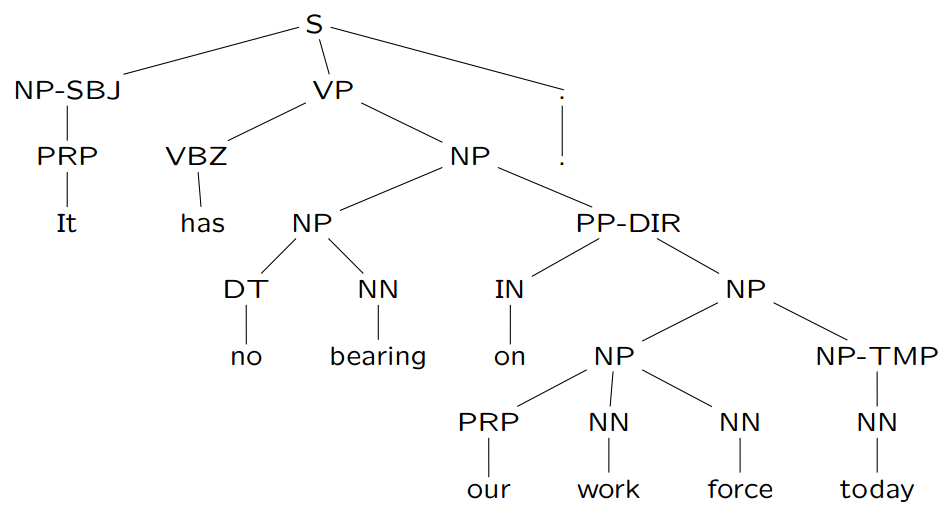
\includegraphics[width=0.6\textwidth]{images/headed-phrase-struct}
  \caption{A headed phrase structure tree}
  \label{fig:headed-phrase-struct-tree}
\end{figure}

In order to convert headed phrase structure trees into dependency trees, we can
use the following algorithm:

\begin{enumerate}
  \item Pick the most important child of each node
  \begin{itemize}
    \item[-] If it's a word, return a leaf node containing the word.
    \item[-] Else, recurse and convert it to a dependency tree
  \end{itemize}
  \item Recurse on all the other children, and make them subtrees of the 
  important child we handled first.
\end{enumerate}

This produces dependency trees that look like what's in
Figure~\ref{fig:converted-dep-tree}.

\begin{figure}[h]
  \centering
  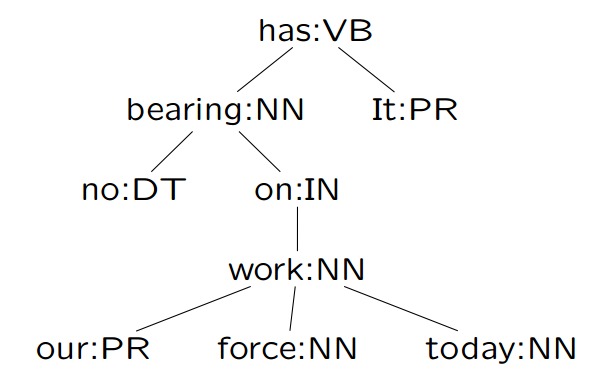
\includegraphics[width=0.4\textwidth]{images/converted-dep-tree}
  \caption{The dependency tree that was derived from the headed phrase structure 
  tree in Figure~\ref{fig:headed-phrase-struct-tree}.}
  \label{fig:converted-dep-tree}
\end{figure}

The last thing we need to think about, is how to pick the most important child
of each node (step 1 of the algorithm). The way to do this is by using a
\textbf{Head Percolation Table (HPT)}. This lists each type of node (`S', `VP'
etc) and lists the order of importance whereby each child node should be ranked.
See Table~\ref{tbl:HPT} for an example.

\begin{table}[h]
  \centering
  \begin{tabular}{|l|l|l|l|}
    \hline
    Root type & Most important & Second most important & \dots \\ \hline
    S & VP & S & \dots\\ \hline
    NP & NN & NNP & \dots\\ \hline
    $\vdots$ & $\vdots$ & $\vdots$ & $\ddots$\\ \hline
  \end{tabular}
  \caption{A sample Head Percolation Table. Its important that the HPC be as 
  accurate as possible, since otherwise the resulting dependency tree will be 
  silly, and it'll make any MALT rules we learn from them silly.}
  \label{tbl:HPT}
\end{table}

\subsection{N-Fold Cross Validation}

N-Fold Cross Validation is a method used to prevent overfitting of Machine
Learning models. Essentially, you split your data into $N$ parts, and train your
model $N$ times. Then, you do $N$ iterations of the training (training on $N-1$
parts each time), and then test on the remaining part. You can then average the
results and thus obtain a reasonable accurate estimate for the error rate of
your model. Figure~\ref{fig:cross-validation} explains this.

\begin{figure}[h]
  \centering
  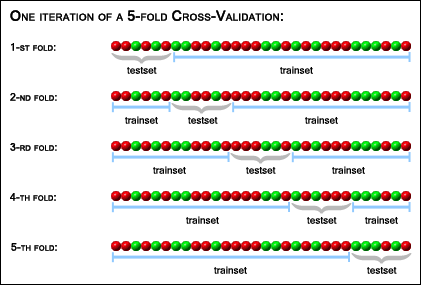
\includegraphics[width=0.7\textwidth]{images/cross-validation}
  \caption{A visual explanation of N-Fold Cross Validation.}
  \label{fig:cross-validation}
\end{figure}

\section{Semantics and Inference}

Given any (normal) piece of text, a reasonably well informed and intelligent
human can figure out, with a variable degree of certainty what the text means.
This section is about confering that skill to computers.

If you had to say what the blanked out word in the following sentence was; ``The
******* saluted crisply to the general as he walked past, his uniform buttons
gleaming'', you'd probably guess `soldier'. But why? Well, we can infer from the
context that it's probably a soldier, since not many other things salute to a
general, or have gleaming buttons. Futhermore, you might have unconciously
realised that it's a noun that fits in the gap (well, it's definately not
something like an adjective), and gotten clues from the length of the missing
word by how many stars there are.

How could we get a computer to solve this problem? Well, one way might be to see
how many of the words in the sentence are associated with soldier; I bet
`general, `salute, `uniform and possibly `crisply'`are all commonly used
whenever `soldier' is used.

To get information about which words commonly occur with which other words, we
can simply go through every word in our dictionary and do the following:

\begin{enumerate}
  \item Use a search engine to find documents about our word.
  \item For each document, remove all instances of our search term.
  \marginpar{This is from an example script I wrote to pull content from the 
  Wikipedia and extract a vector space model. It's on
  \href{https://github.com/Todd-Davies/third-year-notes}{Github} if you want a 
  look... Why don't you submit a pull request while your at it!}
  \item Count the number of occurances of each word, to make a \textbf{Vector 
    Space Model}, something like this:
    \begin{verbatim}
      {'the': 20, 'or': 17, 'of': 16, 'to': 13, 'in': 9, 'are': 8,
       'soldiers': 7, 'from': 7, 'as': 7, 'a': 7, 'Army': 6, 'military': 5,
       'an': 5, 'word': 5, 'and': 5, 'is': 5, 'In': 5, 'term': 4, 'referred': 4,
       'US': 4, 'their': 4, 'Marine': 4, 'other': 4, 'meaning': 4, 'officer': 3,
       'United': 3, 'called': 3, 'service': 3, 'such': 3, 'The': 3, 'States': 3,
       'years': 2, 'soudeour': 2, 'personnel': 2, 'countries': 2, 'because': 2,
       'often': 2, 'employment': 2, 'Latin': 2, 'combat': 2, 'warfighter': 2,
       'by': 2, 'Infantry': 2, 'warfighters': 2, 'occupations': 2, 'French': 2,
       'one': 2, 'armed': 2, 'use': 2, 'type': 2, 'artillery': 2, 'serve': 2...}
    \end{verbatim}
\end{enumerate}

It's also a good idea to stem the words before continuing. For example,
`soldier' and `soldiers' are for all intents and purposes, the same word here.

This information still isn't very useful; we would like a way to compare the
similarity of two vector spaces (i.e. a candidate word, and a document we're
trying to classify).

If you took \texttt{COMP24111}, and you're not half asleep from boredom, then
you might remember a certain method of classification called \textit{nearest
neighbour}. Given a set of n-dimensional vectors and an n-dimensional vector you
want to classify, nearest neighbour will find the distances between all the
vectors in the set, and your other vector, and try to assign it a class based on
the classes of `near' vectors.

This \textit{isn't} what we're going to do here, but it's pretty similar. For
each vector, we can find the cosine of the angle between them:

\[
  \frac{\sum (d_1 \times \dots \times d_n)}
       {\sqrt{\sum (d_0^2) \times \dots \times \sum (d_n^2)}}
\]

The cosine of two vectors is a rough approximation of their similarity. However,
there is an issue; a large document (e.g. an explanation of the Church-Turing
thesis) will have higher values in its vector space than the text off the back
of a chocolate bar, since the former has far more words.

\subsection{TF-IDF}

We don't want document size to affect our similarity measures much, since you
would want a sign posting the way to Manchester to have a high similarity score
to a book about Manchester, but not a high similarity score with a leaflet about
an environmental protest. 

To normalise the vector spaces, we can divide each number in the vector by:

\[
  \sqrt{\sum_{i=1}^ns_i^2}
\]

Where (I think, please correct me if I'm wrong), $s_i$ is the value associated
with the $i$th word in the vector space. This reduces the values in the vector
space proportional to the size of the vector space.

Another thing that makes vector spaces less effective, is the large amount of
noise we get from common words such as `and', `the' and `a'. We want these words
to have less weighting when it comes to determining whether documents are
similar, and possibly give a higher word to more uncommon words such as `marine'
or `howitzer'.

For each word in our dictionary, we could see how many documents it is included
in; this is the \textbf{document frequency}. We could also see how often it
occurs in a single document; the \textbf{term frequency}. We can use these two
values to determine how much we care about each dimension in the vector space,
specifically, we can multiply the vector space value by the term frequency and
then the inverse of the document frequency:

\[
  \text{vector space value} =
    \text{vector space value} \times
    \text{term frequency} \times
    \frac{1}{\text{document frequency}}
\]

This is called the \textbf{TF-IDF} (term frequency - inverse document frequency)
score.

\subsection{Clustering}

Doing the above (document $\rightarrow$ vector space $\rightarrow$ TD-IDF) gets
pretty good results. In the course notes, an example is given where five bacon
themed websites are correctly marked as being more similar than four cricket
themed ones.

The example doesn't get perfect results; it could be improved. To do so, we need
to think back to the Machine Learning course again, and remember \textbf{K-means
clustering}. This is where, given the vector spaces, we try and group documents
into $n$ similar clusters. This is what you do:

\begin{enumerate}
  \item This is where you find the $n$ least similar documents ($n$ = the
    amount of clusters you want to find), and set them as seeds. The logic is
    that these are not similar, and therefore won't be in the same clusters.
  \item For each document, put it in the cluster that has the seed most similar 
    to it.
  \item For each group, find take the weighted average of them all, and make 
    that the new seed. This seed is now called the \textbf{centroid}.
  \item If some documents switched clusters, then go back to step 2 and repeat.
\end{enumerate}

This gets better results than TF-IDF on its own, but still isn't perfect. This
is probably because it only looks at words in isolation. However, as we know
from our Part of Speech tagging exploits, the same word can have different
meanings depending on the \textbf{context} that it appears in. For example,
homonyms can mess up our analysis; we'd like to differentiate between `lead' as
a metal as a verb (``he lead her outside'') and as a noun (``fetch the dog's
lead'').

\marginpar{What if we could cluster the vector space of a word. If there are 
lots of different clusters, then it's probably an ambigous word...}

To do this, we might want to look at the words surrounding a target word, or
possibly think about \textit{syntactically related} words; if two verbs take the
same set of objects, then they're probably similar (e.g. `she kissed him'
$\approx$ `she snogged him').

We can extract information from verb phrase-noun phrase interactions
automatically using regular expressions. For example, the regex \texttt{noun
(MV:verb) det? adj? (OBJ:noun)} will match ``he kissed the beautiful lady'', and
assign \texttt{MV} to `kissed' and \texttt{OBJ} to `lady'.

Since regex matching is fast, we can extract these relationships quickly from
the input corpus.

To see how similar different verbs are, we can do the above for both verbs, and
then intersect what words they are related to. The larger the intersection, the
more related the verbs are. The course notes does this for `read' and `write'.
There are lots of nouns including `book', `letter', `newspaper', `paper',
`music' etc that are related to both words.

However, while obviously `read' and `write' are related, they're (in a sense)
antonyms too. See, we are able to cluster words this way, but we can't tell
\textit{how} the words are related. Are they synonyms (kiss/snog), antonyms
(eat/regurgitate) etc?

Furthermore, the analysis is quite dumb, and is easily confused by sentences
that aren't `simple' or require a context to understand properly. Again, the
course notes give a good example; you might devour a book, and an intergalactic
monster might devour a world, which presents issues if you're trying to cluster
`devour' with `eat', which is obviously related.

\subsubsection{Choosing cluster poiints}

So, although we've decided that our measures for detecting whether words are
similar are rather dumb, we know they do work. So, how do we start using them to
cluster similar words together? As mentioned above, to do K-means clustering, we
need to both decide on how many seeds to create (which will give us the same
number of clusters) and which elements to set as the initial seeds.

We're going to cheat regarding the number of seeds we'll create, since it's hard
to do automatically. For choosing the seeds though, there is a nice way of doing
things:

\begin{enumerate}
  \item For 0 to $n$
  \begin{enumerate}
    \item Pick $m$ random seeds 
    \item Calculate their \textit{density}, which is the sum of their pairwise 
      cosines.
  \end{enumerate}
  \item Choose the set of seeds that had the lowest density.
\end{enumerate}

This works because if the sum of pairwise cosines is low, that means the items
were dissimilar, which is likely to give us seeds that properly represent the
clusters that they will go on to form.

In practice, the choice of seeds is important, but not vital; it is possible for
the initial seed to move out of the cluster it initially created. Obviously
better seeds will make the algorithm converge faster and make it less likely
that silly clusters will result.

A good idea is to run the algorithm many times with steadily increasing seed
sizes, and select the number of seeds that gives the maimum average density in
the clusters (except from when the number of clusters is close to the number of
words, since then the average density will be 1!).

\subsection{Hand Coded Relations}

The trouble we're having now is that we know when concepts are related, but not
how they're related. For example, we can tell that two sentences are related
(e.g. `I drove the car' and `I drove a fiat'), but not how they're related; is
driving a fiat the opposite of driving a car, is it better than driving a car?

In order to solve this problem, we're going to need to create (or obtain some
data that our algorithms can use to help distinguish between words. WordBanks
have \textbf{Synsets}, which are collecitons of the different senses of words.
This lets us get a list of potential meanings for a word in a sentence, like
this (but in a different format obviously):

\begin{description}
  \item \textbf{Run:}
  \begin{mymulticols}
    \begin{itemize}
      \item On the run
      \item Run across a friend
      \item Run around in the field
      \item Run for president
      \item Many more...
    \end{itemize}
  \end{mymulticols}
\end{description}

Synset relationships (superset and opposite relations) are also given. This is
most useful to us, since we can see what items other items are linked to.
Obviously the relations aren't always good; sometimes you get ones that seem
completely arbitrary, but you can use synset relations so do things like:

\[
  \text{I melted the ice} \rightarrow \text{The ice is no longer frozen}
\] 

\subsection{Word Sense Disambugation}

We can use the \textbf{Page Rank} algorithm to decide on what interpretation of
each word is correct. Page Rank is (was, I expect that its evolved quite a bit
now) the algorithm that powers Google search. The idea is that we can think of
synsets just like webpages. Synsets relate one word to a collection of related
words, and web pages are related to other web pages via links.

\subsubsection{Page Rank}

Page rank works by using the \textit{random surfer model}, which is the
assumption that a web surfer will click random links on a web page to get to
other web pages (each link has a $\frac{1}{n}$ chance of being clicked).

We can use a markov model to represent this; where the probability of the user
being on web page $x$ at time $t + 1$ is equal to the sum of the probability of
them being on a web page with a link to $x$ at time $t$ multiplied by the
probability of them clicking the link to $x$:

\[
  prob(\text{Web Page}_x^{t + 1}) =
    \sum (prob(\text{Web Page}_i^t) + prob(S_i \rightarrow S_x))
\]

If you construct a weighted graph representing the web pages and their
connections, and simulate the time increasing, then eventually, you will find a
convergence, so long as the following criteria hold:

\begin{itemize}
  \item All web pages must have at least one working link (i.e. no inescapable
    webpages).
  \item No inescapable loops.
\end{itemize}

If one of these criteria is not met, then the model will converge to zero. This
is an issue, since we can't always guarentee that our input web pages will
conform to these rules. See the course notes (p309-314) for an example of the
convergance.

We can also supply a damping parameter for some page, which is the chance that a
surfer will visit it. Then, the chance of visiting other pages linked by a page
is $\frac{1 - damping}{n}$.

You can `personalise' results by reserving some probability at each stage,
dividing it by the pages you're biased towards (e.g. web pages of bands you
like). This has \textit{the effect of making those pages more important, as well
as making the pages linked too by those pages more important too}.

\subsubsection{Application of Page Rank to Synsets}

As you might have guessed, the reason we looked at Page Rank, is that you can
apply it to synsets just like you can between web pages. It works for
synset/superset links and between synsets and the synsets of words that appear
inside it.

Given a word we want to find more about, we can get its definition, and then get
the synsets of the open class words in the definition. For example, if `run' was
defined as `moving faster than a walk', we could get the synsets for `move',
`fast' and `walk' (this is called a \textit{gloss}). If we ran Page Rank on a
graph consisting of those words (+ `run'), then we'd get the most prominent
synsets for `run'. If we personalise the Page Rank by making the synsets that
appear in whatever text you're analysing more weighty, then we'll get better
results.

Two big advantages of using synsets and page rank, is that they disambugate all
the words in a phrase in one pass, so they're not too slow. Furthermore, since
we have relatively good word banks, somebody doesn't have to spend ages coming
up with and inputting lots of different senses of different words.

% p343
